\documentclass{book}

\usepackage{listings}
\usepackage{theorem}
\usepackage{graphicx}
\usepackage{hyperref}
\usepackage{amsfonts}
\usepackage{amsmath}
\usepackage[table]{xcolor}
\usepackage{array,calc}
\usepackage{amsmath}

\newtheorem{exercise}{Exercise}


\lstset{
  language=Java,
  basicstyle=\ttfamily\footnotesize,
  numbers = left
}

\newcommand{\co}[1]{\lstinline[language=Java, basicstyle=\ttfamily]{#1}}

\begin{document}

\chapter{ImageJ}
ImageJ is a Java library for digital image analysis and processing. The library contains interfaces and classes for creating, modifying and displaying images. In this chapter, we explain how to perform basic image operations using this library.

\section{Setting up ImageJ}\label{sec:imagej-setup}
ImageJ is a library for \emph{Java}. In the remainder of this section, we assume that a Java Development Kit (version 6 or higher) and the Eclipse integrated development environment are installed on your machine. If Java is not installed on your machine, download and install a Java Development Kit from \href{http://www.oracle.com/technetwork/java/javase/downloads/index.html}{http://www.oracle.com/technetwork/java/javase/downloads/index.html}. Similarly, if the Eclipse IDE is not installed on your machine, download and install it from \href{http://www.eclipse.org/}{http://www.eclipse.org/}.

The ImageJ implementation, tutorials and additional documentation are available online at \href{http://rsbweb.nih.gov/ij}{http://rsbweb.nih.gov/ij}. To install ImageJ, download the platform independent release from \href{http://rsbweb.nih.gov/ij/download.html}{http://rsbweb.nih.gov/ij/download.html}. Extract the zip file to a location of your choice.

ImageJ can be used both as a standalone application and as a library. To run the application,  execute ImageJ.exe (on Windows) or ImageJ.app (on Mac). After starting the application, the following graphical user interface should be displayed on your screen:

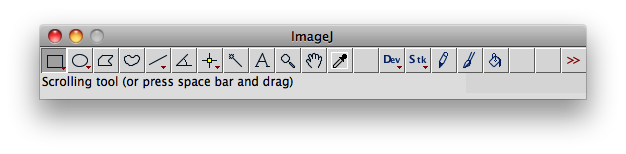
\includegraphics[scale=0.5]{ImageJ-screenshot.png}

\begin{exercise}
Experiment with the ImageJ graphical user interface:
\begin{itemize}
  \item Open \texttt{lena.png} via \texttt{File>Open...}.
  \item \texttt{lena.png} is an rgb color image. However, we will first explain most image processing techniques using grayscale images. Convert the image to 8 bit grayscale via \texttt{Image>Type>8-bit}.
  \item A grayscale image is a function from coordinates to colors in the range 0 to 255. Visualise this function via  \texttt{Plugins>3D>Interactive 3D Surface Plot}. 
  \item Detect edges in the image via \texttt{Process>Find Edges}. Later in this course, we will explain how edge detection works and how it can be used to sharpen images and to perform seam carving.
\end{itemize} 
\end{exercise}

The ImageJ library is packaged as a jar file called \texttt{ij.jar}. This jar file is located in the ImageJ directory. To use the interfaces and classes provided by ImageJ, \texttt{ij.jar} must be included in the classpath when compiling and running any program that uses the library. 

\begin{exercise}
Set up Eclipse as follows:
\begin{itemize}
  \item Start Eclipse and create a new Java project called \texttt{digitalimageprocessing}.
  \item Add \texttt{ij.jar} to the classpath by right-clicking the project and selecting \texttt{Build Path>Add External Archives ...} as shown below.
  \begin{center}
  \includegraphics[scale=0.25]{eclipse-classpath.png}
  \end{center}
  After adding \texttt{ij.jar} to the classpath, the project should contain a new item called \texttt{Referenced Libraries}. This item contains \texttt{ij.jar} as a subitem. 
  \item To access the ImageJ API documentation directly in Eclipse, right-click \texttt{ij.jar} in Eclipse and select \texttt{Properties} and click \texttt{Javadoc Location}. Enter \href{http://rsbweb.nih.gov/ij/developer/api/}{http://rsbweb.nih.gov/ij/developer/api/} as the \texttt{Javadoc location path} and click \texttt{OK}.  
\end{itemize}
\end{exercise}

\section{Images}
An image is a rectangular, two-dimensional grid of pixels, where each pixel represents the color at that location. In ImageJ, images are represented as objects of the class \texttt{ImagePlus}. This class provides methods for querying the image's width, height, type, pixel values, etc.

\subsection{Opening images}
The first step in most image processing applications is loading one or more images into memory. The Java standard library provides the method \co{ImageIO.read} for this purpose. The code snippet shown below illustrates loading an image into memory: 
\begin{lstlisting}
File file = new File("lena.png");
BufferedImage inMemoryImage = ImageIO.read(file);
ImagePlus image = new ImagePlus(file.getName(), inMemoryImage);
\end{lstlisting}
\co{ImageIO.read} throws an \co{IOException} when reading fails.  For example, this occurs when the given file does not exist, it is not a valid image or if the user does not have permission to read the file.

ImageJ supports a number of different image types: 8-bit grayscale, 16-bit grayscale, 32-bit floating-point grayscale, 8-bit indexed color and 32-bit RGB color. The class \co{ImagePlus} contains a constant (i.e. a final static field) for each such type. For example, \co{GRAY8} is the constant corresponding to 8-bit grayscale, while \co{COLOR\_256} is the constant corresponding to 32-bit RGB color. In this course, we will mostly be making use of 8-bit grayscale and 32-bit RGB color images. The type of an \co{ImagePlus} object can be queried by calling the method \co{getType}. 

For the code snippet shown above to compile, import statements must be added to the class containing this code. For example, the classes \co{File} and \co{IOException} are part of the package \co{java.io}, while \co{ImagePlus} is part of \co{ij}.

\begin{exercise}\label{ex:myfirstimageprocessor}.
Open an image and display its size and type. To do so, create a new class named \texttt{MyFirstImageProcessor} in the default package. Add a \texttt{main} method to this class that first opens \texttt{lena.png} and then prints the image's width, height and type using respectively the methods \co{getWidth}, \co{getHeight}, \co{getType}. If opening the file fails, the program should not crash, but an error message should be displayed.
\end{exercise}

The method \co{ImageIO.read} is overloaded such that it can not only read images from files on disk, but also from arbitrary urls. For example,  the following code snippet opens \co{mysteryimage.png} from the given url.
\begin{lstlisting}
URL url = new URL("http://www.cs.kuleuven.be/~jans/mysteryimage.png");
BufferedImage inMemoryImage = ImageIO.read(url);
ImagePlus image = new ImagePlus(url.getFile(), inMemoryImage);
\end{lstlisting}

\begin{exercise}
Modify \texttt{MyFirstImageProcessor} from exercise~\ref{ex:myfirstimageprocessor} such that it displays information about \co{mysteryimage.png} instead of \co{lena.png}.
\end{exercise}

\subsection{Displaying images}
Images can be displayed via an \texttt{ImageWindow} as follows:
\begin{lstlisting}
ImagePlus image = ...;
ImageWindow window = new ImageWindow(image);
window.setVisible(true);
\end{lstlisting}
\begin{exercise}
Make the \texttt{main} method of the class \texttt{MyFirstImageProcessor} display the image in a window.
\end{exercise}

\subsection{Modifying images}
Images can be modified via an \texttt{ImageProcessor}. The key methods of this class are \texttt{getPixel} and \texttt{putPixel}. These methods respectively return and modify the pixel value (as an integer) at a given location. For grayscale images, the pixel value is an integer in the range 0 (representing black) to 255 (representing white). For RGB color images, the pixel value is the integer encoding of the separate color components.  For example, the code snippet shown below inverts a grayscale image. That is, white pixels become black and vice versa, black pixels become white.

\begin{lstlisting}
ImagePlus image = ...;
ImageProcessor ip = image.getProcessor();
for(int x = 0; x < ip.getWidth(); x++) {
  for(int y = 0; y < ip.getHeight(); y++) {
    int grayColor = ip.getPixel(x, y);
    ip.putPixel(x, y, 255 - grayColor);
  }  
}
\end{lstlisting}

Note that modifying an \co{ImagePlus} via an \co{ImageProcessor} only affects the data stored in memory. The image file where the data was originally read is not modified by \co{putPixel}. In Section~\ref{sec:saving-images}, we will explain how to save modified images to disk.

\begin{exercise}\label{ex:invert}
Write a class \texttt{ImageInvertor} that inverts grayscale images based on the code snippet shown on above. The output for \texttt{lena-gray.png} should look as follows:
\begin{center}
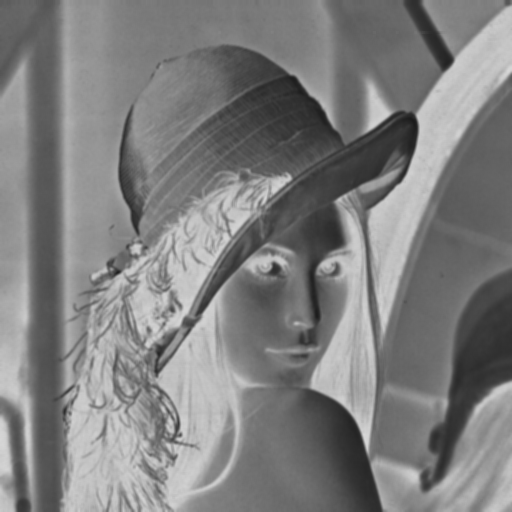
\includegraphics[scale=0.2]{lena-gray-inverted.png}
\end{center}
\end{exercise}

\begin{exercise}\label{ex:flipper}
Write a class  \texttt{ImageFlipper} that flips an image vertically (i.e. puts the image upside down). For example, the output for \texttt{lena.png} should look as follows:
\begin{center}
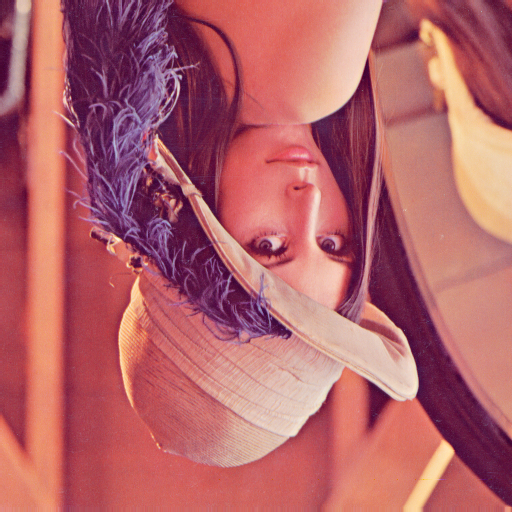
\includegraphics[scale=0.2]{lena-flipped-hor.png}
\end{center}
\end{exercise}

\begin{exercise}
Modify the class \texttt{ImageInvertor} from Exercise~\ref{ex:invert} such that it can handle RGB color images.
\begin{itemize}
  \item Write a method \co{getRGBComponentsFromInt} that converts an integer into an array containing the RGB components.
  \item Write a method \co{getIntFromRGBComponents} that converts an array of RGB components into an integer.
  \item Modify the \texttt{main} method of \texttt{ImageInvertor}  such that it checks whether the image is 8-bit grayscale or RGB color. You can use the method \co{getType} to determine the image type. If the image is grayscale, the existing code should be used for inverting the image. If the image is RGB color, then for each pixel each color component should be inverted separately. For example, if the RGB components of a pixel are (255, 0, 50), then the inverted pixel value is (0, 255, 205). If the image is neither 8-bit grayscale or RGB color, print an error message. Use the methods \co{getRGBComponentsFromInt} and \co{getIntFromRGBComponents} to help you out.
\end{itemize}
The output of \texttt{ImageInvertor} for \texttt{lena.png} should look as follows:
\begin{center}
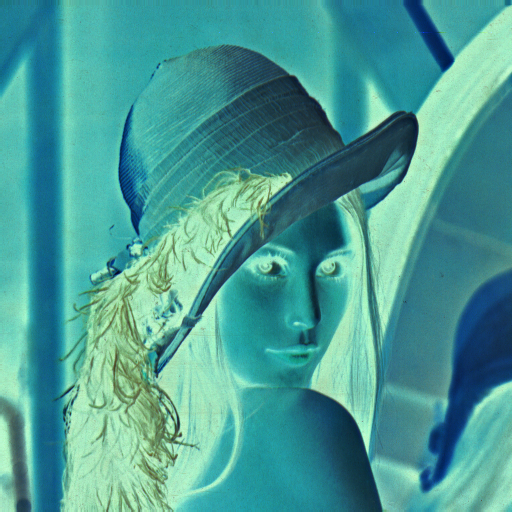
\includegraphics[scale=0.2]{lena-inverted.png}
\end{center}
\end{exercise}

\begin{exercise}
What value does \co{getPixel} return if the given coordinate is out of range? What about \co{putPixel}? What happens when \co{putPixel} is called on an 8-bit grayscale image and the given color is outside of the range 0-255? Look this up in the documentation of the class \href{http://rsbweb.nih.gov/ij/developer/api/ij/process/ImageProcessor.html}{\co{ImageProcessor}}.
\end{exercise}

\subsection{Saving images}\label{sec:saving-images}
In addition to displaying images on screen, we often want to save them to disk. The code shown below makes use of the static method \co{ImageIO.write} to save \co{img} to \co{output.png} in the png file format.
\begin{lstlisting}
ImagePlus img = ...;
ImageIO.write(img.getBufferedImage(), "png", 
  new File("output.png"));
\end{lstlisting}
Note that \texttt{ImageIO.write} throws \texttt{IOException} when writing the image fails. For example, writing can fail because the current user does not have write permission or because the file is in use by another application.

\begin{exercise}\label{ex:imageflipper2}
Modify the class \texttt{ImageFlipper} from Exercise~\ref{ex:flipper} such that it saves the flipped image to disk to \texttt{out.png}. The application should not crash when \co{ImageIO.write} fails, but instead write an error message to standard output (i.e.  \texttt{System.out}).
\end{exercise}

\subsection{Creating new images}
The class \co{NewImage} contains a number of static methods for creating images. For example, the code shown below creates a new grayscale image named ``myImageName'' with width 400 and height 300. All pixels are initially black.
\begin{lstlisting}
ImagePlus image = NewImage.createByteImage(
  "theImageName", 400, 300, 1, NewImage.FILL_BLACK);
\end{lstlisting}
RGB color images can be created via the static method \co{createRGBImage}.

\begin{exercise}\label{ex:gradient-image}
Write a class \co{CreateGradientImage} that generates a \emph{gradient} grayscale image. The size of this new image is 256 x 100. Pixels in the \co{i}th column should have color \co{i}. Save the image to disk or display it on screen. The resulting image should look as follows:

\begin{center}

\includegraphics[scale=0.3]{gradient-image.png}
\end{center}

Can you generate a similar image if the width is not exactly 256 pixels?
\end{exercise}

\begin{exercise}
Write a class \co{CreateRGBGradientImage} that generates a 256x256 gradient RGB color image containing the colors red and blue. That is, the pixel at position \co{(x, y)} must be assigned the rgb color whose red component is equal to x, whose green component is equal to 0 and whose blue component is equal to y. The resulting image should look as follows:

\begin{center}
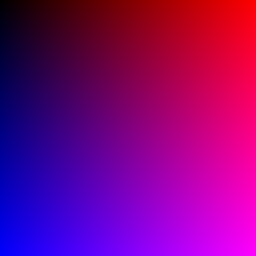
\includegraphics[scale=0.3]{rgb-gradient.png}
\end{center}

Can you generate a similar image if the size is not exactly 256x256?
\end{exercise}

\section{Getting user input}
In all but the simplest applications, user input is required. For example, the user can typically select the image to be processed and set the parameters of the image processing operation.

\subsection{Command line arguments}
A simple way to allow users to customize the behaviour of a program is using command-line arguments. As an example, consider the class \co{EchoNTimes} shown below. 
\begin{lstlisting}
class EchoNTimes {
  public static void main(String[] args) {
    if(args.length != 2) {
      System.out.println("2 arguments expected");
      return;
    }
    String text = args[0];
    int n;
    try {
      n = Integer.parseInt(args[1]); 
    } catch(NumberFormatException ex) {
      System.out.println("not a number: " + args[2]);
      return;     
    }
    for(int i = 0; i < n; i++) {
      System.out.println(text);    
    }
  }
}
\end{lstlisting}
This class prints a given string a certain number of times. For example, the output of the command
\begin{verbatim}
java EchoNTimes hello 3
\end{verbatim}
is
\begin{verbatim}
hello
hello
hello
\end{verbatim}
In Java, the command line arguments are passed to the \co{main} method as an array of \co{String}s via the \co{args} parameter. That is, \co{args.length} denotes the number of command line arguments and \co{args[i]} denotes the \co{i}th argument. For the command shown above, \co{args.length} is two, args[0] equals ``hello'' and args[1] equals ``3''. In lines 3 to 6, \co{EchoNTimes} checks that the user provides exactly two arguments. In line 7, the first argument is stored in the variable \co{text}. The second command line argument is converted to an integer via \co{Integer.parseInt} in lines 8 to 14. The method \co{Integer.parseInt} throws a \co{NumberFormatException} if the given string is not a number. \co{EchoNTimes} catches this potential exception via the try-catch block and prints an error message. Finally, the given text is printed n times in lines 15 to 17.

Note that each primitive type in Java has a corresponding class. Each such class has a static method to convert a \co{String} to that type. As shown in the example above, the class \co{Integer} has the method \co{parseInt}. Similarly, the class \co{Double} has a method \co{parseDouble} and the class \co{Boolean} has a method \co{parseBoolean}.

In Eclipse, command-line arguments can be passed to a program by clicking \texttt{Run>Run Configurations ...} and editing the \texttt{Program arguments} field as shown below:

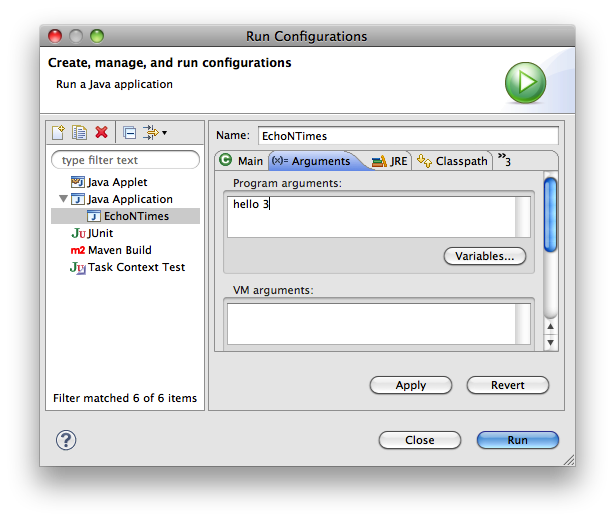
\includegraphics[scale=0.5]{arguments-eclipse.png} 

\begin{exercise}\label{ex:imageflipper3}
Modify the class \co{ImageFlipper} from Exercise~\ref{ex:imageflipper2} such that the input and output image can be passed as command line arguments. For example, the command
\begin{verbatim}
java ImageFlipper stevejobs.jpg steve-flipped.jpg 
\end{verbatim}
should flip the image of Steve Jobs upside down and saves the resulting image to \co{steve-flipped.jpg}.
\end{exercise}

\subsection{Standard input}
Many programs do not only require user input when they start but also during their execution. For this purpose, mainstream operating systems such as Windows, Mac and Linux attach two streams to each process, one for reading data called standard input and one for writing data called standard output. In Java, these streams can respectively be accessed via the static fields \co{System.in} and \co{System.out}. For example, text can be written to standard out via \co{System.out.println}. Text can be read from standard input using a \co{Scanner}.

The class \co{Scanner} provides methods such \co{nextInt}, \co{nextDouble}, \co{nextLine} and \co{nextBoolean} to read several types of data from an \co{InputStream}. The program shown below displays a given string a certain number of times. However, the string and the number are not passed to the program as command line arguments, but via standard input.

\begin{lstlisting}
class EchoNTimesUsingScanner {
  public static void main(String[] args) {
    Scanner scanner = new Scanner(System.in);
    String text; int n;
    try {
    	System.out.println("Which line?");
    	text = scanner.nextLine();
    	System.out.println("How many times?");
    	n = scanner.nextInt();
    } catch(NoSuchElementException ex) {
    	System.out.println("invalid input");
    	return;
    }
    for(int i = 0; i < n; i++) {
      System.out.println(text);    
    }
  }
}
\end{lstlisting}

If \co{EchoNTimesUsingScanner} is executed on command line, the interaction looks as follows:

\begin{verbatim} 
$ java EchoNTimes
Which line?
hello
How many times?
3
hello
hello
hello
\end{verbatim}

Note that all \co{Scanner.nextX} methods throw \co{NoSuchElementException} if the input does not match the expected type.

\subsection{GenericDialog}
Graphical user interfaces are an alternative to command line arguments and reading from standard input. For example, one may want to display the window shown below to acquire input from the user.  

\begin{center}
\includegraphics[scale=0.5]{generic-dialog.png}
\end{center}

How can we do this in ImageJ? The code shown below uses a \co{GenericDialog} to acquire input from the user. In line 3, a new \co{GenericDialog} with title \co{Echo-N-Times} is created. In lines 4 and 5, a text  and a number input field is added to the dialog. The method \co{showDialog} in line 6 displays the dialog and blocks until the user presses either Cancel or Ok.  If the user pressed Cancel, \co{main} returns in lines 7 and 8. Lines 9 and 10 then store the data entered in dialog into local variables. 

\begin{lstlisting}
public class EchoNTimesUsingGenericDialog {
  public static void main(String[] args) {
    GenericDialog dialog = new GenericDialog("Echo-N-Times");
    dialog.addStringField("Text:", "default text");
    dialog.addNumericField("Number of times:", 3, 0);
    dialog.showDialog();
    if(dialog.wasCanceled())
      return;
    String text = dialog.getNextString();
    int n = (int) dialog.getNextNumber();
    for(int i = 0; i < n; i++) {
      System.out.println(text);    
    }
  }
}
\end{lstlisting}

\begin{exercise}
Modify the class \co{CreateGradientImage} from Exercise~\ref{ex:gradient-image} such that the user can enter the width, height and name of the output image and the direction of the gradient (either left-to-right or top-to-bottom) into a \co{GenericDialog}. 

\begin{center}
\includegraphics[scale=0.5]{gradient-generic-dialog.png}
\end{center}

You can use \co{GenericDialog.addChoice} to allow to user to select the desired direction from a drop down menu. 
\end{exercise}

Next to \co{GenericDialog}, you can use arbitrary arbitrary Swing components to get input from the user. For example, \co{java.swing.JFileChooser} allows the user to browse his or her file system for a file, while \co{java.swing.JColorChooser} allows selecting a color.

%What happens if you set the color to -1 for a grayscale image?
%What happens if you get or put a pixel outside of the image?

\section{ImageJ Plugins}
The ImageJ application can be extended with plugins. A plugin is a Java class that implements the interface \co{ij.plugin.filter.PlugInFilter}. This interface defines two methods: \co{setup} and \co{run} that must be implemented by the plugin. The \co{run} method is the core of the plugin that performs the actual work. However, when using a \co{PlugInFilter}, ImageJ first calls the \co{setup} method (before calling \co{run}) to check that the plugin supports the given image type. For example, consider the plugin \co{InvertorPlugin_} shown below.

\begin{lstlisting}
public class InvertorPlugin_ implements PlugInFilter {
  @Override
  public void run(ImageProcessor ip) {
    for(int x = 0; x < ip.getWidth(); x++) {
      for(int y = 0; y < ip.getHeight(); y++) {
        ip.putPixel(x, y, 255 - ip.getPixel(x, y));
      }
    }
  }
  
  @Override
  public int setup(String args, ImagePlus imp) {
    return DOES_8G;  
  }
}
\end{lstlisting}

The goal of this plugin is to invert a grayscale image. The return value of \co{setup} indicates that the plugin only supports grayscale images as it returns \co{DOES_8G} (\texttt{8G} is a shorthand for 8-bit grayscale). The plugin does not support any other image types such as RGB color. The \co{run} method does the actual work of inverting each pixel.

To run a plugin within ImageJ, perform the following steps:
\begin{itemize}
  \item The ImageJ application contains a folder called \texttt{plugins}. This folder already contains a number of plugins. Create a new subdirectory \texttt{myplugins} of \texttt{plugins}. All your plugins will be placed in this directory.
  \item Copy the java file (e.g. \texttt{InvertorPlugin\_.java}) containing your plugin to \texttt{myplugins}. Make sure that the class you are copying is in the default package.
  \item Start the ImageJ application and open an image. Convert this image to a type supported by the plugin via the \texttt{Image>Type} menu.
  \item In the ImageJ application, click \texttt{Plugins>Compile and run ...} and select the java file you just copied. The plugin is now compiled and executed on the image. 
\end{itemize}

\begin{exercise}
Write a plugin that modifies the color of rows of pixels.
\begin{itemize}
  \item Write a plugin \co{WhiteLinesPlugin\_} that makes every other line in a grayscale or color image white. The output of the plugin on \texttt{lena.png} should look as follows:

\begin{center}
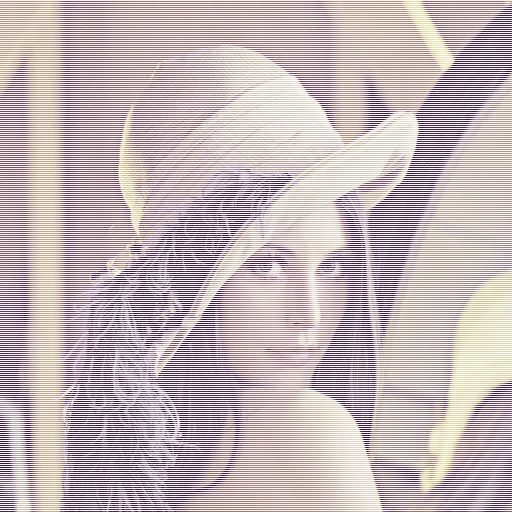
\includegraphics[scale=0.2]{lena-white-lines.png}
\end{center}

\item Modify \co{WhiteLinesPlugin\_} such that the user enter in a dialog how many normal lines the plugin should place between every white line.

\item \textbf{Extra} Use a \co{JColorChooser} to allow the user to select the color of the lines.
\end{itemize}
\end{exercise}

\begin{exercise}
While modifying the pixels in an image, you can update the corresponding \co{ImageWindow} by calling \co{image.updateAndDraw()}. Write a plugin \co{ScrollPlugin\_} that scrolls an images vertically. For \texttt{lena.png}, the user should see (amongst others) the following images:

\begin{center}
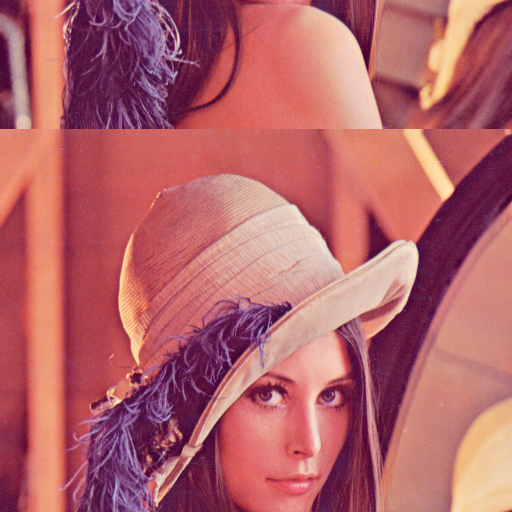
\includegraphics[scale=0.2]{lena-scrolled-1.png} 
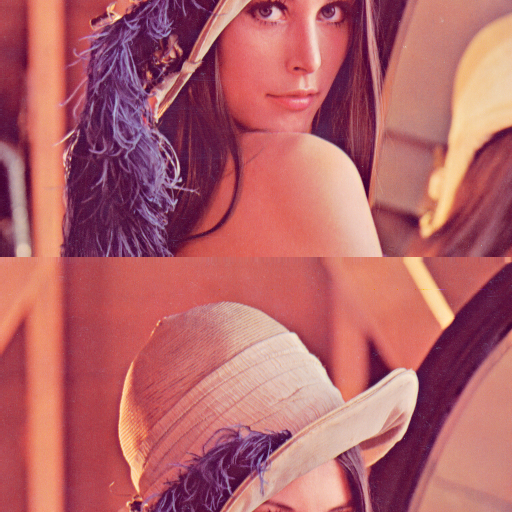
\includegraphics[scale=0.2]{lena-scrolled-2.png}
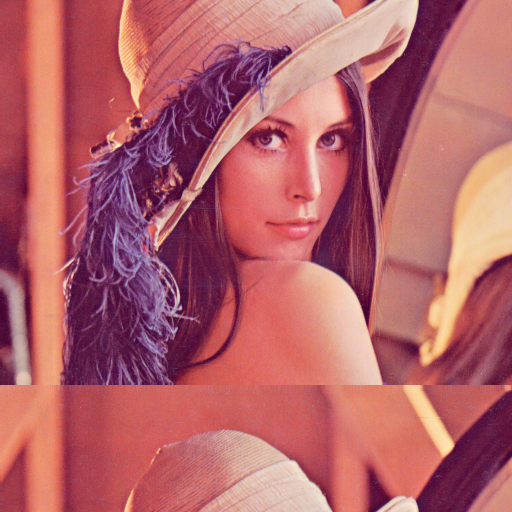
\includegraphics[scale=0.2]{lena-scrolled-3.png}
\end{center}
\end{exercise}

\begin{exercise}
Write an ImageJ plugin that creates a border around a grayscale image. The user should be able to select the border width and color via sliders in a \co{GenericDialog}. 

\begin{center}
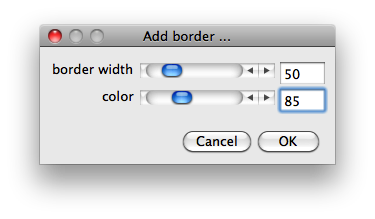
\includegraphics[scale=0.5]{sliders.png}
\end{center}

The method \co{GenericDialog.addSlider} adds a slider to a dialog. The selected value can be retrieved via \co{getNextNumber}. For example, the output of your plugin for \co{lena.png} should look as follows when the user sets the border width equal to 50 and the color equal to 85:
 
\begin{center}
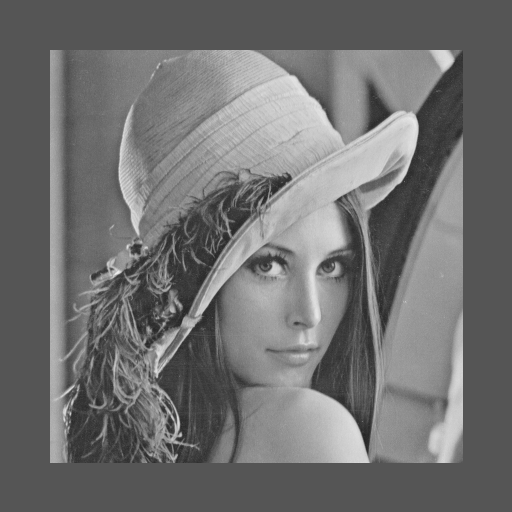
\includegraphics[scale=0.2]{lena-border.png}
\end{center}
\end{exercise}

\begin{exercise}
Write an ImageJ plugin to display only a single color component of an RGB color image. For example, to only display the red component, set the green and blue components of each pixel to 0 (but do not modify the red component). Displaying only the red, green and blue component of \co{lena.png} should look as follows:
 
\begin{center}
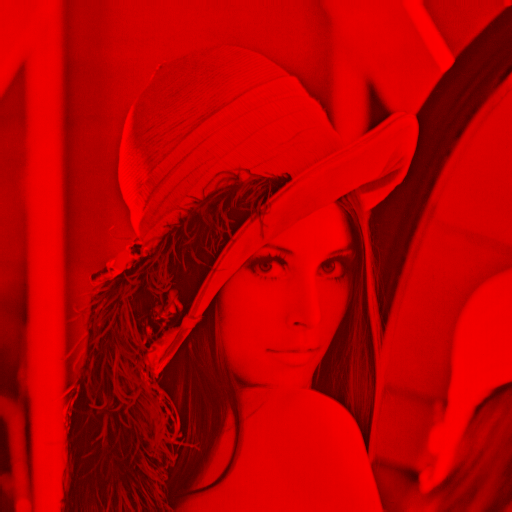
\includegraphics[scale=0.2]{lena-onlyred.png}
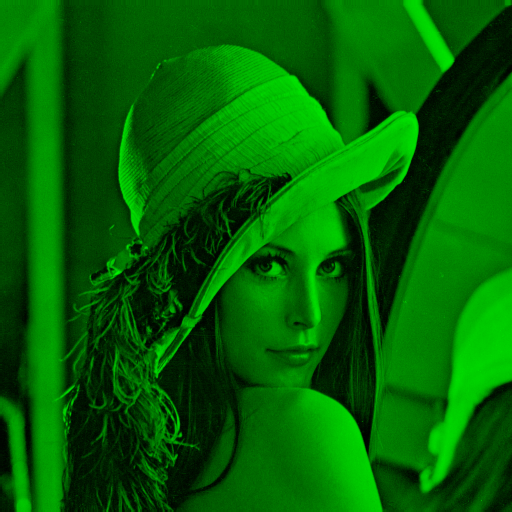
\includegraphics[scale=0.2]{lena-onlygreen.png}
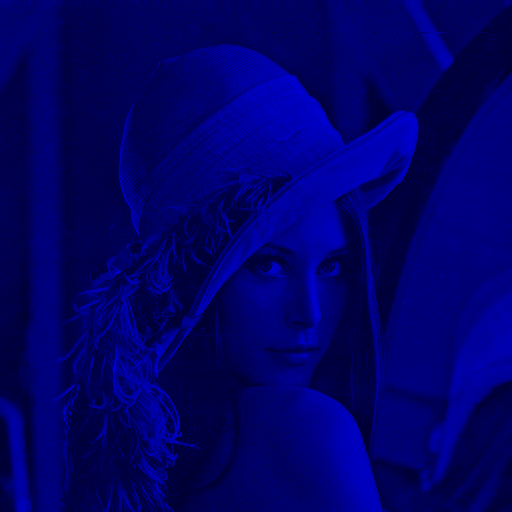
\includegraphics[scale=0.2]{lena-onlyblue.png}
\end{center}
What is the expected outcome if you run this plugin on \co{red.png} selecting green as the component to be shown?
\end{exercise}

% live preview?, progress bar?

% access exif info in IJ?
\end{document}